\documentclass[10pt,twocolumn]{article}

% Packages
\usepackage[utf8]{inputenc}
\usepackage[T1]{fontenc}
\usepackage{graphicx}
\usepackage{booktabs}
\usepackage{amsmath}
\usepackage{amssymb}
\usepackage{hyperref}
\usepackage{geometry}
\usepackage{caption}
\usepackage{subcaption}
\usepackage{algorithm}
\usepackage{algorithmic}
\usepackage{tikz}
\usetikzlibrary{shapes,arrows,positioning,fit,backgrounds}

\geometry{margin=0.75in}

% Title
\title{\textbf{Attention-Based Multi-Modal Fusion for Drug Synergy Prediction}}
\author{Kusal Debnath}
\date{January 2026}

\begin{document}

\maketitle

% Abstract
\begin{abstract}
Drug combination therapy is a promising strategy for treating complex diseases, but identifying synergistic drug pairs remains challenging due to the vast combinatorial space. We present an end-to-end deep learning model that predicts drug synergy by learning to fuse multi-omics cell line profiles with molecular drug representations through attention mechanisms. Our model employs a trainable omics encoder that processes mRNA, miRNA, and proteomics data, combined with pre-trained MolFormer embeddings for drug molecules. Using cross-attention, the model learns how drug pairs interact with cellular contexts to produce synergistic effects. Experiments on the DrugComb dataset demonstrate consistent improvement during training, achieving a validation MSE of 13.40 on the Synergy\_ZIP score prediction task.
\end{abstract}

% ============================================================================
\section{Introduction}
% ============================================================================

Drug combination therapy has emerged as a critical approach in treating complex diseases such as cancer, where single-agent treatments often fail due to drug resistance and tumor heterogeneity \cite{drugcomb}. The key challenge lies in identifying which drug combinations exhibit synergistic effects---where the combined effect exceeds the sum of individual effects.

Computational prediction of drug synergy can significantly accelerate the drug discovery process by narrowing down the vast combinatorial space of possible drug pairs. This task requires integrating heterogeneous information: (1) molecular properties of the drugs, and (2) the biological context of the target cell line.

In this work, we propose an attention-based multi-modal fusion architecture that:
\begin{itemize}
    \item Learns meaningful representations from raw multi-omics data (mRNA, miRNA, proteomics)
    \item Leverages pre-trained molecular language models for drug representations
    \item Uses cross-attention to model drug-cell line interactions
    \item Trains end-to-end for synergy score prediction
\end{itemize}

% ============================================================================
\section{Problem Formulation}
% ============================================================================

Given a drug pair $(d_1, d_2)$ and a cell line $c$ characterized by multi-omics profiles, we aim to predict the synergy score $y \in \mathbb{R}$ that quantifies the degree of synergistic interaction.

Formally, let:
\begin{itemize}
    \item $\mathbf{s}_1, \mathbf{s}_2$: SMILES representations of drugs $d_1$ and $d_2$
    \item $\mathbf{x}_{\text{mRNA}} \in \mathbb{R}^{23808}$: mRNA expression profile
    \item $\mathbf{x}_{\text{miRNA}} \in \mathbb{R}^{627}$: miRNA expression profile  
    \item $\mathbf{x}_{\text{prot}} \in \mathbb{R}^{3171}$: Proteomics profile
    \item $y$: Synergy score (ZIP, Bliss, Loewe, or HSA)
\end{itemize}

Our goal is to learn a function $f: (\mathbf{s}_1, \mathbf{s}_2, \mathbf{x}_{\text{mRNA}}, \mathbf{x}_{\text{miRNA}}, \mathbf{x}_{\text{prot}}) \rightarrow y$.

% ============================================================================
\section{Dataset}
% ============================================================================

We use the \textbf{DrugComb} dataset \cite{drugcomb}, a comprehensive resource for drug combination studies containing high-throughput screening data across multiple cancer cell lines.

\subsection{Dataset Statistics}

\begin{table}[h]
\centering
\caption{Dataset split statistics}
\label{tab:dataset}
\begin{tabular}{@{}lrr@{}}
\toprule
\textbf{Split} & \textbf{Samples} & \textbf{Percentage} \\
\midrule
Training & 207,968 & 70.0\% \\
Validation & 29,710 & 10.0\% \\
Test & 59,420 & 20.0\% \\
\midrule
\textbf{Total} & \textbf{297,098} & 100\% \\
\bottomrule
\end{tabular}
\end{table}

\subsection{Feature Dimensions}

\begin{table}[h]
\centering
\caption{Input feature dimensions}
\label{tab:features}
\begin{tabular}{@{}llr@{}}
\toprule
\textbf{Modality} & \textbf{Source} & \textbf{Dimension} \\
\midrule
Drug Embedding & MolFormer-XL & 768 \\
mRNA Expression & Cell Line & 23,808 \\
Proteomics & Cell Line & 3,171 \\
miRNA Expression & Cell Line & 627 \\
\bottomrule
\end{tabular}
\end{table}

\subsection{Target Variable}

We predict the \textbf{Synergy\_ZIP} score, which quantifies synergy using the Zero Interaction Potency (ZIP) model. The ZIP score represents the deviation from expected additive effects:
\begin{itemize}
    \item $\text{ZIP} > 0$: Synergistic interaction
    \item $\text{ZIP} = 0$: Additive interaction
    \item $\text{ZIP} < 0$: Antagonistic interaction
\end{itemize}

% ============================================================================
\section{Model Architecture}
% ============================================================================

Our model consists of four main components: (1) Drug Encoder, (2) Omics Fusion Model, (3) Cross-Attention Fusion, and (4) Prediction Head.

\begin{figure}[h]
\centering
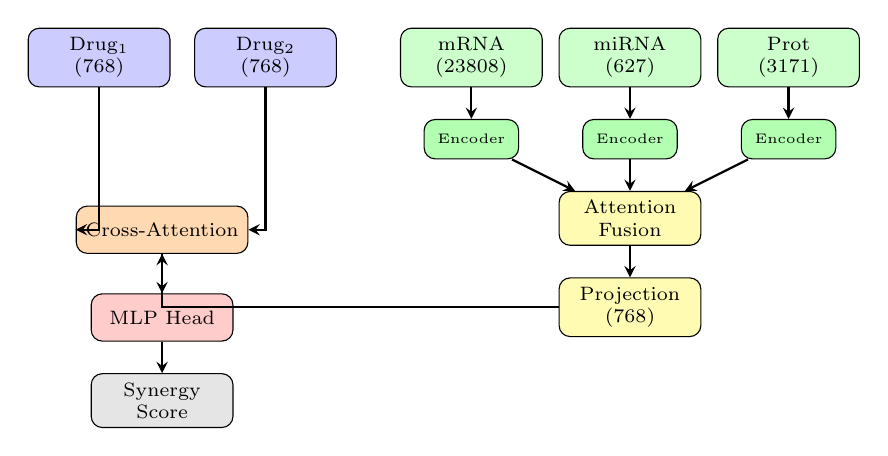
\begin{tikzpicture}[
    node distance=0.5cm,
    box/.style={rectangle, draw, rounded corners, minimum width=1.8cm, minimum height=0.6cm, align=center, font=\scriptsize},
    smallbox/.style={rectangle, draw, rounded corners, minimum width=1.2cm, minimum height=0.5cm, align=center, font=\tiny},
    arrow/.style={->, >=stealth, thick}
]

% Drug inputs
\node[box, fill=blue!20] (d1) {Drug$_1$\\(768)};
\node[box, fill=blue!20, right=0.3cm of d1] (d2) {Drug$_2$\\(768)};

% Omics inputs
\node[box, fill=green!20, right=0.8cm of d2] (mrna) {mRNA\\(23808)};
\node[box, fill=green!20, right=0.2cm of mrna] (mirna) {miRNA\\(627)};
\node[box, fill=green!20, right=0.2cm of mirna] (prot) {Prot\\(3171)};

% Omics encoders
\node[smallbox, fill=green!30, below=0.4cm of mrna] (enc1) {Encoder};
\node[smallbox, fill=green!30, below=0.4cm of mirna] (enc2) {Encoder};
\node[smallbox, fill=green!30, below=0.4cm of prot] (enc3) {Encoder};

% Omics fusion
\node[box, fill=yellow!30, below=0.4cm of enc2] (fusion) {Attention\\Fusion};

% Projection
\node[box, fill=yellow!30, below=0.4cm of fusion] (proj) {Projection\\(768)};

% Cross attention
\node[box, fill=orange!30, below=1.5cm of d1, xshift=0.8cm] (cross) {Cross-Attention};

% Prediction head
\node[box, fill=red!20, below=0.5cm of cross] (head) {MLP Head};

% Output
\node[box, fill=gray!20, below=0.4cm of head] (out) {Synergy\\Score};

% Arrows
\draw[arrow] (mrna) -- (enc1);
\draw[arrow] (mirna) -- (enc2);
\draw[arrow] (prot) -- (enc3);
\draw[arrow] (enc1) -- (fusion);
\draw[arrow] (enc2) -- (fusion);
\draw[arrow] (enc3) -- (fusion);
\draw[arrow] (fusion) -- (proj);
\draw[arrow] (d1) |- (cross);
\draw[arrow] (d2) |- (cross);
\draw[arrow] (proj) -| (cross);
\draw[arrow] (cross) -- (head);
\draw[arrow] (head) -- (out);

\end{tikzpicture}
\caption{SynergyModel architecture overview}
\label{fig:architecture}
\end{figure}

\subsection{Drug Encoder (Frozen)}

Drug molecules are represented using \textbf{MolFormer-XL} \cite{molformer}, a large-scale molecular language model pre-trained on 1.1 billion molecules. Given a SMILES string, MolFormer produces a 768-dimensional embedding capturing molecular structure and properties. These embeddings are pre-computed and frozen during training.

\subsection{Omics Fusion Model (Trainable)}

The omics encoder processes three modalities independently before fusing them:

\subsubsection{Modality-Specific Encoders}
Each omics modality is processed by a dedicated encoder with batch normalization:
\begin{equation}
\mathbf{e}_m = \text{Linear}(\text{ReLU}(\text{BN}(\text{Linear}(\text{BN}(\mathbf{x}_m)))))
\end{equation}
where $m \in \{\text{mRNA}, \text{miRNA}, \text{prot}\}$ and $\mathbf{e}_m \in \mathbb{R}^{256}$.

\subsubsection{Attention-Based Fusion}
The three 256-dimensional embeddings are stacked and processed through multi-head self-attention:
\begin{equation}
\mathbf{E} = [\mathbf{e}_{\text{mRNA}}; \mathbf{e}_{\text{miRNA}}; \mathbf{e}_{\text{prot}}] \in \mathbb{R}^{3 \times 256}
\end{equation}
\begin{equation}
\mathbf{e}_{\text{fused}} = \text{MeanPool}(\text{MultiHeadAttn}(\mathbf{E}, \mathbf{E}, \mathbf{E}))
\end{equation}

\subsubsection{Projection Attention}
The fused 256-dimensional embedding is projected to 768 dimensions using a learned query attention mechanism to match the drug embedding space.

\subsection{Cross-Attention Fusion}

Drug embeddings and omics embedding are combined via self-attention to learn drug-cell line interactions:
\begin{equation}
\mathbf{S} = [\mathbf{d}_1; \mathbf{d}_2; \mathbf{o}] \in \mathbb{R}^{3 \times 768}
\end{equation}
\begin{equation}
\mathbf{f} = \text{LayerNorm}(\mathbf{S} + \text{Dropout}(\text{MultiHeadAttn}(\mathbf{S})))
\end{equation}
\begin{equation}
\mathbf{z} = \text{MeanPool}(\mathbf{f}) \in \mathbb{R}^{768}
\end{equation}

\subsection{Prediction Head}

A three-layer MLP with dropout predicts the synergy score:
\begin{equation}
\hat{y} = \text{Linear}(\text{ReLU}(\text{Linear}(\text{ReLU}(\text{Dropout}(\text{Linear}(\mathbf{z}))))))
\end{equation}

\subsection{Model Statistics}

\begin{table}[h]
\centering
\caption{Model configuration}
\label{tab:model}
\begin{tabular}{@{}lr@{}}
\toprule
\textbf{Component} & \textbf{Value} \\
\midrule
Total Parameters & 20,432,557 \\
Trainable Parameters & 20,432,557 \\
Embedding Dimension & 768 \\
Hidden Dimension (Omics) & 256/512 \\
Attention Heads (Fusion) & 4 \\
Attention Heads (Cross) & 8 \\
Dropout Rate & 0.1--0.2 \\
\bottomrule
\end{tabular}
\end{table}

% ============================================================================
\section{Experiments}
% ============================================================================

\subsection{Training Configuration}

\begin{table}[h]
\centering
\caption{Training hyperparameters}
\label{tab:training}
\begin{tabular}{@{}lr@{}}
\toprule
\textbf{Hyperparameter} & \textbf{Value} \\
\midrule
Optimizer & AdamW \\
Learning Rate & $1 \times 10^{-4}$ \\
Batch Size & 64 \\
Epochs & 100 \\
Loss Function & MSE \\
Device & NVIDIA GPU (CUDA) \\
\bottomrule
\end{tabular}
\end{table}

\subsection{Results}

\begin{table}[h]
\centering
\caption{Training results (MSE Loss)}
\label{tab:results}
\begin{tabular}{@{}lrrr@{}}
\toprule
\textbf{Metric} & \textbf{Initial} & \textbf{Final} & \textbf{Best} \\
\midrule
Train Loss & 22.63 & 11.66 & 11.66 \\
Val Loss & 21.31 & 13.40 & 13.40 \\
\bottomrule
\end{tabular}
\end{table}

\begin{figure}[h]
\centering
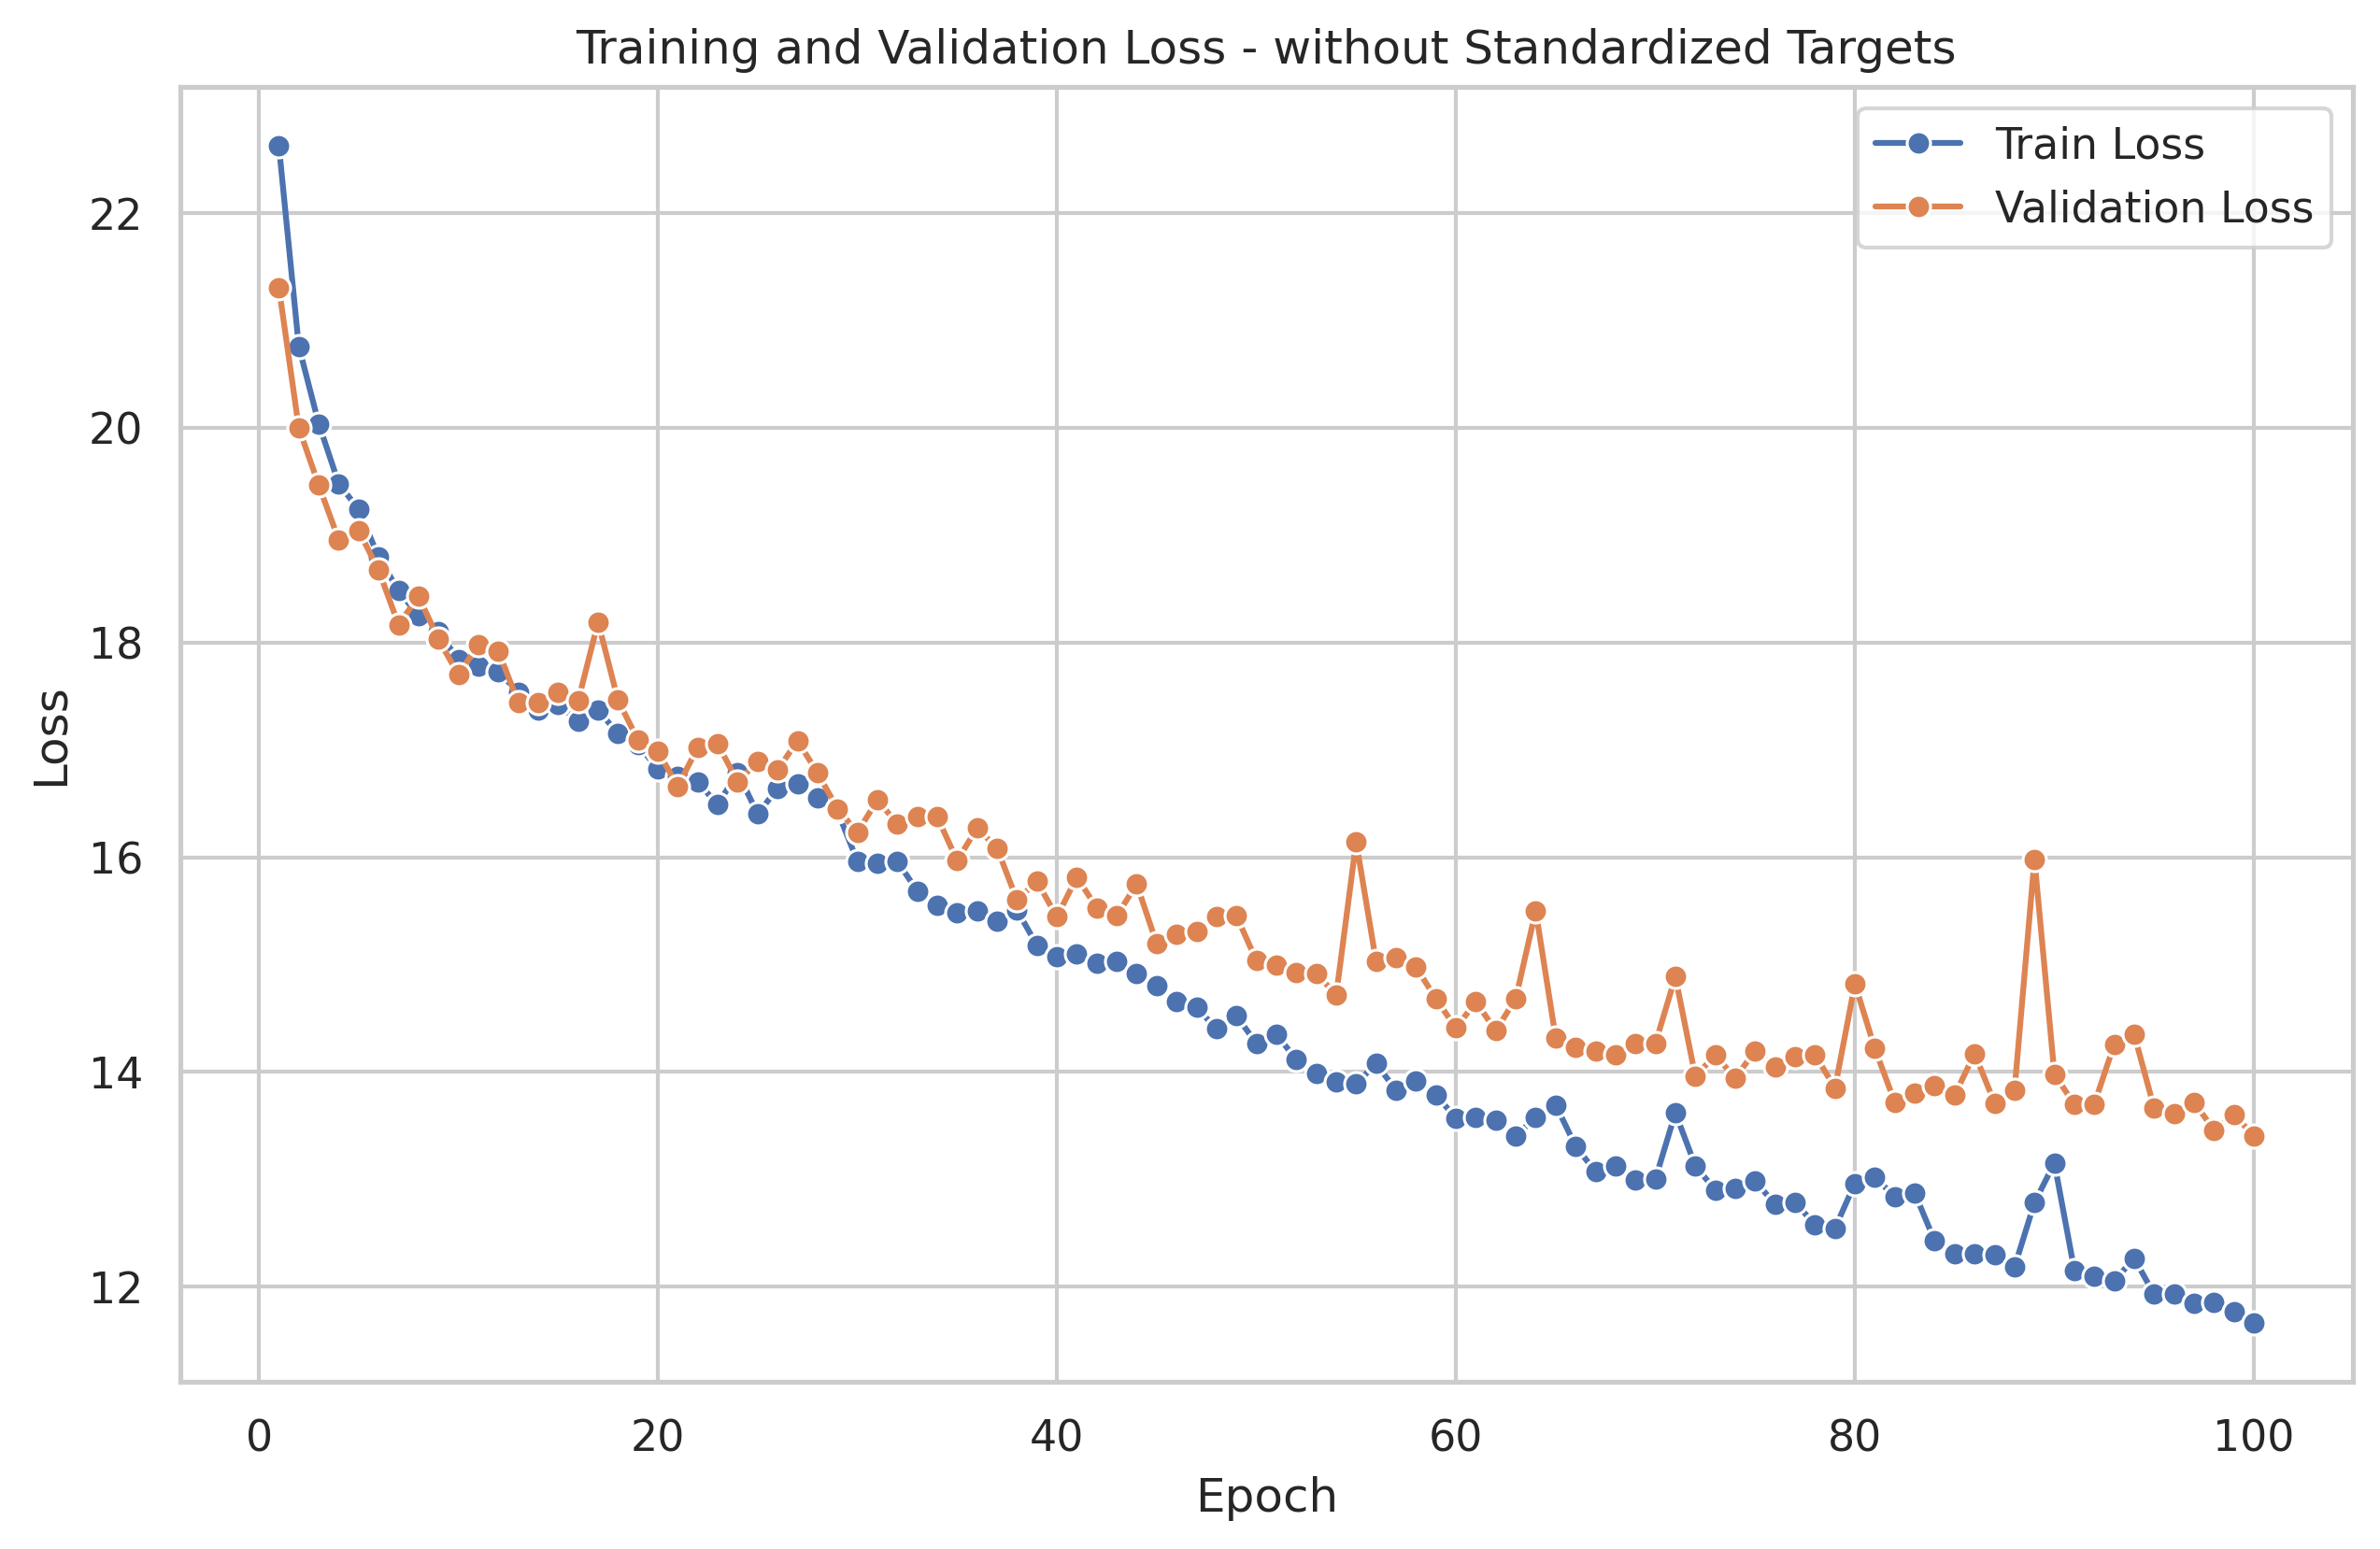
\includegraphics[width=0.9\columnwidth]{../logs/synergy_attn_20260119_233831/loss_plot_wo_std.png}
\caption{Training and validation loss curves over 100 epochs}
\label{fig:loss}
\end{figure}

\subsection{Analysis}

Key observations from training:

\begin{enumerate}
    \item \textbf{Consistent Improvement}: Both training and validation loss decreased steadily, with validation MSE improving from 21.31 to 13.40 (37\% reduction).
    
    \item \textbf{Generalization Gap}: The gap between training (11.66) and validation (13.40) loss suggests mild overfitting, which could be addressed with regularization.
    
    \item \textbf{Training Stability}: The model showed stable convergence without significant oscillations, validating our architecture choices including BatchNorm in omics encoders.
    
    \item \textbf{Training Time}: ~1 minute per epoch on GPU, totaling approximately 1.7 hours for 100 epochs.
\end{enumerate}

% ============================================================================
\section{Discussion}
% ============================================================================

\subsection{Strengths}

\begin{itemize}
    \item \textbf{End-to-End Learning}: Unlike approaches that pre-compute fixed omics embeddings, our model learns task-specific representations optimized for synergy prediction.
    
    \item \textbf{Multi-Modal Fusion}: The attention-based fusion allows the model to learn which omics modalities are most informative for specific drug-cell line combinations.
    
    \item \textbf{Interpretability Potential}: Attention weights can be extracted to understand which drugs/omics features contribute to predictions.
    
    \item \textbf{Scalability}: The architecture can accommodate additional omics modalities or drug features.
\end{itemize}

\subsection{Limitations}

\begin{itemize}
    \item \textbf{Single Synergy Metric}: Currently trained only on ZIP scores; other metrics (Bliss, Loewe, HSA) may provide complementary information.
    
    \item \textbf{Cell Line Generalization}: Performance on unseen cell lines not yet evaluated.
    
    \item \textbf{No Target Standardization}: Synergy scores were not standardized, which may affect optimization dynamics.
\end{itemize}

% ============================================================================
\section{Next Steps}
% ============================================================================

\subsection{Immediate Improvements}

\begin{enumerate}
    \item \textbf{Target Standardization}: Normalize synergy scores to have zero mean and unit variance for more stable training.
    
    \item \textbf{Multi-Task Learning}: Predict all four synergy metrics (ZIP, Bliss, Loewe, HSA) simultaneously with shared representations.
    
    \item \textbf{Regularization}: Add weight decay, increase dropout, or use early stopping to reduce overfitting.
    
    \item \textbf{Learning Rate Scheduling}: Implement cosine annealing or reduce-on-plateau for better convergence.
    
    \item \textbf{Test Set Evaluation}: Evaluate final model on held-out test set with additional metrics (MAE, $R^2$, Pearson/Spearman correlation).
\end{enumerate}

\subsection{Architecture Enhancements}

\begin{enumerate}
    \item \textbf{Deeper Omics Encoders}: Add more layers or use residual connections for better feature extraction.
    
    \item \textbf{Drug-Drug Interaction Module}: Explicit modeling of drug-drug interactions before cell line fusion.
    
    \item \textbf{Graph Neural Networks}: Replace MolFormer with GNNs that can be fine-tuned end-to-end on molecular graphs.
    
    \item \textbf{Transformer Layers}: Stack multiple cross-attention layers for deeper drug-omics interactions.
\end{enumerate}

\subsection{Data Augmentation}

\begin{enumerate}
    \item \textbf{Drug Pair Symmetry}: Exploit $(d_1, d_2) \equiv (d_2, d_1)$ for data augmentation.
    
    \item \textbf{Noise Injection}: Add Gaussian noise to omics features during training.
    
    \item \textbf{Mixup}: Interpolate between samples for regularization.
\end{enumerate}

% ============================================================================
\section{Implementation Plan}
% ============================================================================

\subsection{Phase 1: Evaluation \& Baseline (Week 1)}

\begin{itemize}
    \item[\checkmark] Implement end-to-end SynergyModel with attention fusion
    \item[\checkmark] Train on DrugComb dataset
    \item[$\square$] Evaluate on test set with comprehensive metrics
    \item[$\square$] Compare against simple MLP baseline (concatenation)
    \item[$\square$] Analyze attention weights for interpretability
\end{itemize}

\subsection{Phase 2: Model Improvements (Week 2--3)}

\begin{itemize}
    \item[$\square$] Implement target standardization
    \item[$\square$] Add learning rate scheduling (CosineAnnealing)
    \item[$\square$] Multi-task learning for all synergy metrics
    \item[$\square$] Hyperparameter tuning (hidden dims, attention heads, dropout)
    \item[$\square$] Cross-validation for robust performance estimates
\end{itemize}

\subsection{Phase 3: Advanced Features (Week 4--5)}

\begin{itemize}
    \item[$\square$] Implement drug pair symmetry augmentation
    \item[$\square$] Add GNN-based drug encoder option
    \item[$\square$] Stacked transformer layers for deeper fusion
    \item[$\square$] Cell line embedding via graph (if tissue/mutation data available)
\end{itemize}

\subsection{Phase 4: Analysis \& Documentation (Week 6)}

\begin{itemize}
    \item[$\square$] Comprehensive ablation studies
    \item[$\square$] Interpretability analysis (attention visualization)
    \item[$\square$] Error analysis on prediction failures
    \item[$\square$] Final paper preparation
\end{itemize}

% ============================================================================
\section{Conclusion}
% ============================================================================

We presented an attention-based multi-modal fusion model for drug synergy prediction that learns to integrate multi-omics cell line profiles with molecular drug representations in an end-to-end fashion. Our model achieves a validation MSE of 13.40 on the DrugComb dataset, demonstrating the effectiveness of attention mechanisms for modeling drug-cell line interactions. Future work will focus on multi-task learning, architectural improvements, and comprehensive evaluation on held-out test data.

% ============================================================================
% References
% ============================================================================

\begin{thebibliography}{9}

\bibitem{drugcomb}
Zagidullin, B., et al. (2019). DrugComb: an integrative cancer drug combination data portal. \textit{Nucleic Acids Research}, 47(W1), W43--W51.

\bibitem{molformer}
Ross, J., et al. (2022). Large-Scale Chemical Language Representations Capture Molecular Structure and Properties. \textit{Nature Machine Intelligence}, 4, 1256--1264.

\bibitem{attention}
Vaswani, A., et al. (2017). Attention is All You Need. \textit{NeurIPS}.

\bibitem{zip}
Yadav, B., et al. (2015). Searching for Drug Synergy in Complex Dose-Response Landscapes Using an Interaction Potency Model. \textit{Computational and Structural Biotechnology Journal}, 13, 504--513.

\end{thebibliography}

\end{document}
